\subsection{ERM}
\underline{To show:} ERM is strictly consistent for $\Lambda$ 
\begin{equation} \label{1}
	\Rightarrow \lim_{p \rightarrow \infty}  
		P\Big\{ \Big| R_{(\vec{w}_p)} - 
			R_{(\vec{w}_0)} \Big|
			\geq \eta
		\Big\} = 0
\end{equation}
\underline{Proof:} From the definition of the strict consistency it follows that
\begin{equation} 
	\lim_{p \rightarrow \infty}  
		P\Big\{ R_{\mathrm{emp} (\vec{w}_p)}^{(P)}
			\geq R_{(\vec{w}_0)} + 
			\frac{\varepsilon}{2}
		\Big\} = 0, \forall \varepsilon > 0
\end{equation}
Let $\Lambda_{ \big(R_{(\vec{w}_0)} + \varepsilon\big) }$ be
\begin{equation}
	\Lambda_{ \big(R_{(\vec{w}_0)} + \varepsilon\big) }
	= \Big\{ \vec{w}: R_{(\vec{w})} 
	\geq R_{(\vec{w}_0)} + \varepsilon \Big\}
\end{equation}
\begin{center}
	\includegraphics[width=11cm]{proofERMconsistency}
\end{center}
From the definition of strict consistency it follows that
\begin{equation}
	\lim_{p \rightarrow \infty}  
		P\Bigg\{ \inf_{\vec{w} \in 
			 \Lambda_{ \big(R_{ (\vec{w}_0) }  
				+ \varepsilon\big) } } 
			R_{\mathrm{emp} (\vec{w})}^{(P)}
			\geq R_{(\vec{w}_0 )} 
				+ \frac{\varepsilon}{2}
		\Bigg\} = 1
\end{equation}
because $\Lambda_{ \big(R_{(\vec{w}_0)} + \varepsilon\big) }$ only contains $\vec{w}$ for which $R_{ \vec{w} } \geq R_{ \vec{w}_0} + \varepsilon$ holds.
Therefore 
\begin{equation}
	\lim_{p \rightarrow \infty}  
		P\bigg\{ \vec{w}_p \in 
			\Lambda_{ \big(R_{(\vec{w}_0) } 
				+ \varepsilon \big) }
		\bigg\} = 0
\end{equation}
and
\begin{equation}
	R_{ (\vec{w}_0 )} \leq R_{ (\vec{w}_p )}
	\leq R_{ (\vec{w}_0 ) } + \varepsilon 
	\text{ for } \vec{w}_p 
		\notin  \Lambda_{ \big(R_{(\vec{w}_0 
				+ \varepsilon)} \big) }
\end{equation}
can be concluded, which shows that (\ref{1}) holds.
